\newpage
\section{Attack of Ferro-Tartaglia}

You may recall that the Ferro-Tartaglia method gives 
\[
\sqrt[3]{\frac{-1+\sqrt{-31}}{2}} + \frac{2}{\sqrt[3]{\frac{1}{2}(-1+\sqrt{-31})}}
\]
as a solution to: $y = x^3-6x+1$. Moreover, as this plot of $y = x^3-6x+1$ shows
\[
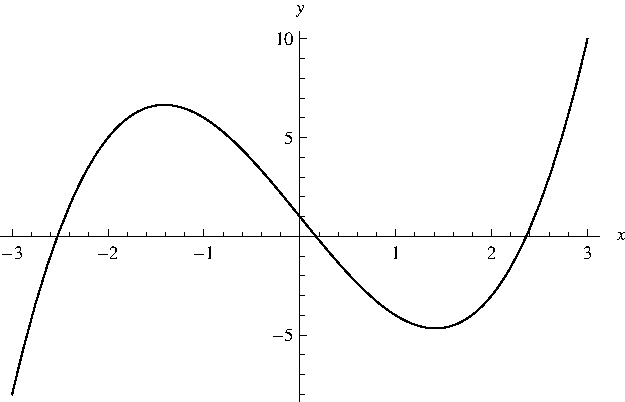
\includegraphics[width=3in]{../graphics/cubicPlot.pdf}
\]
this must be a real solution\dots But how? There is a square-root of a
negative number in the expression above! Ok, uncharacteristically for
me, I'll show you how this is done. Please fasten your seat belts and
place your trays in the upright position.

Start by looking at:
\[
\frac{-1+\sqrt{-31}}{2} = \frac{-1}{2} + \frac{\sqrt{31}}{2} i 
\]
If we plot this in the complex plane, we get:
\[
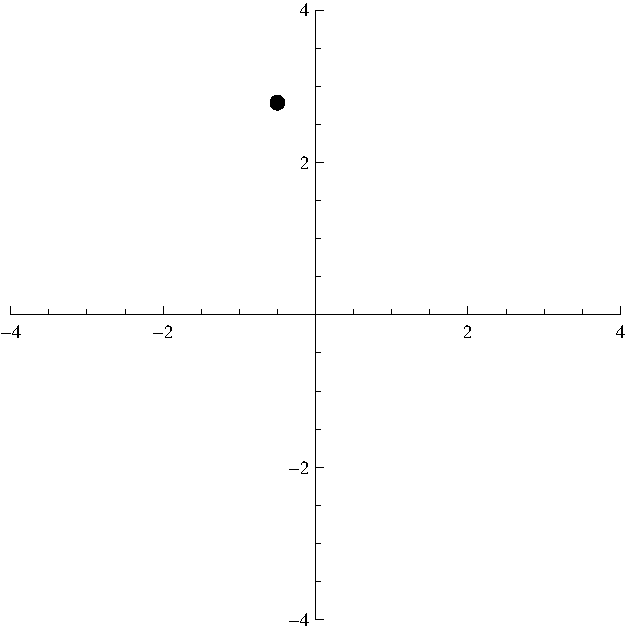
\includegraphics[width=3in]{../graphics/CmplxPlane1.pdf}
\]
Using the distance formula, we see:
\[
\sqrt{\left( \frac{-1}{2} \right)^2 + \left(\frac{31}{2}\right)^2} = 2\sqrt{2}
\]
Hence we can plot the point $\left(\frac{-1}{4\sqrt{2}}, \frac{31}{4\sqrt{2}}\right)$ on the unit circle:
\[
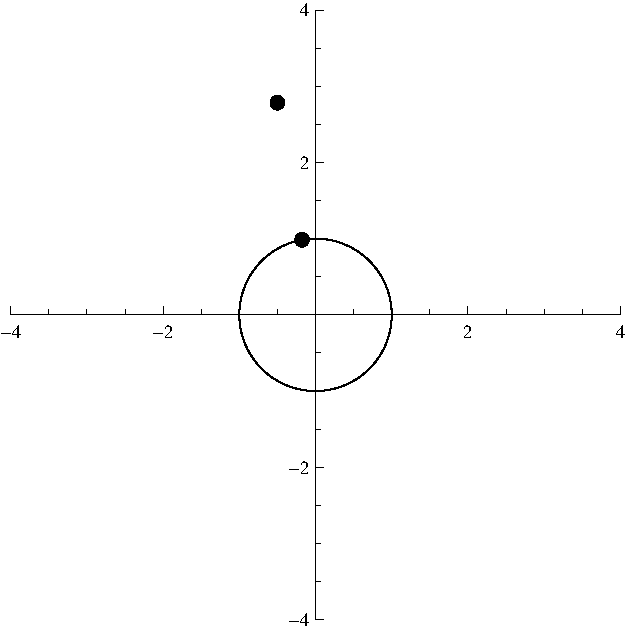
\includegraphics[width=3in]{../graphics/CmplxPlane2.pdf}
\]
Since multiplication of complex numbers lying on the unit circle in the
complex plane is simply rotation, the cube-root of $\frac{-1}{2} +
\frac{31}{2} i$ is:
\[
\left(\sqrt[3]{2\sqrt{2}}\right)\cos\left(\arcsin\left(\frac{31}{4\sqrt{2}}\right)/3\right) + i \left(\sqrt[3]{2\sqrt{2}}\right) \sin\left( \arcsin\left(\frac{31}{4\sqrt{2}}\right)/3\right)
\]
Gosh, that's a mess, plotted on the complex plane, it looks like the black point below:
\[
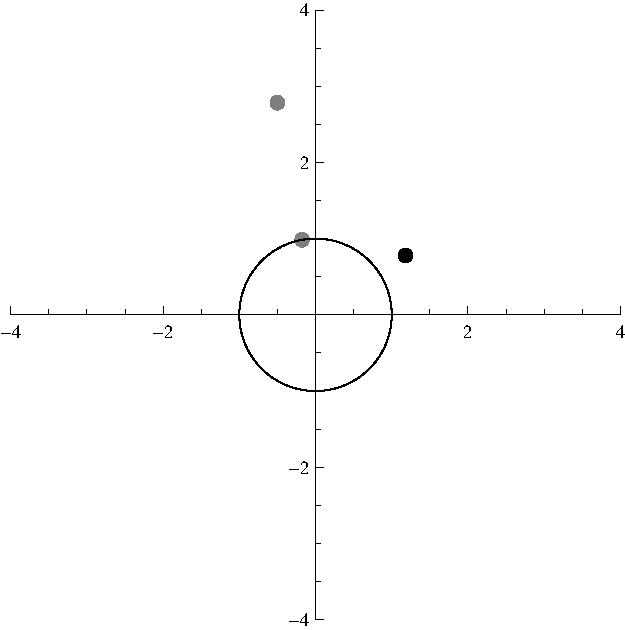
\includegraphics[width=3in]{../graphics/CmplxPlane3.pdf}
\]

Now we'll compute the cube-root of: 
\begin{align*}
\frac{8}{\frac{1}{2}(-1+\sqrt{-31})} = \frac{-1}{2} + \frac{-\sqrt{31}}{2} i 
\end{align*}
If we plot this in the complex plane, we get:
\[
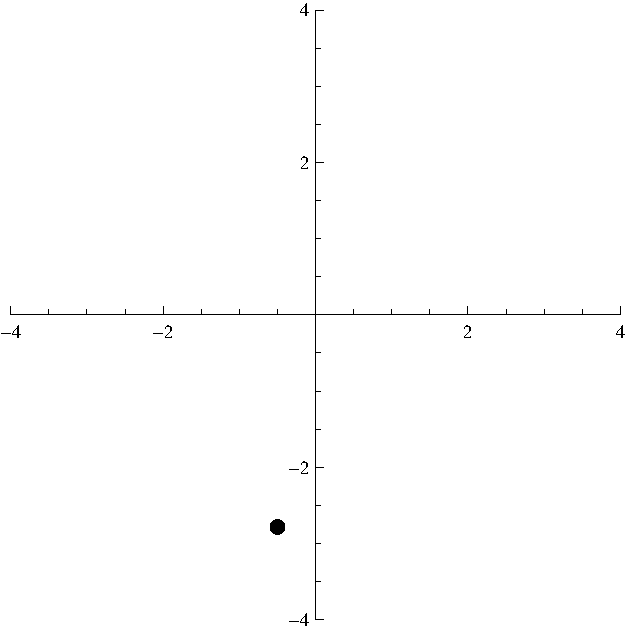
\includegraphics[width=3in]{../graphics/CmplxPlane4.pdf}
\]
Again, using the distance formula, we see:
\[
\sqrt{\left( \frac{-1}{2} \right)^2 + \left(\frac{31}{2}\right)^2} = 2\sqrt{2}
\]
Hence we can plot the point $\left(\frac{-1}{2}, \frac{-\sqrt{31}}{2} \right)$ on the unit circle:
\[
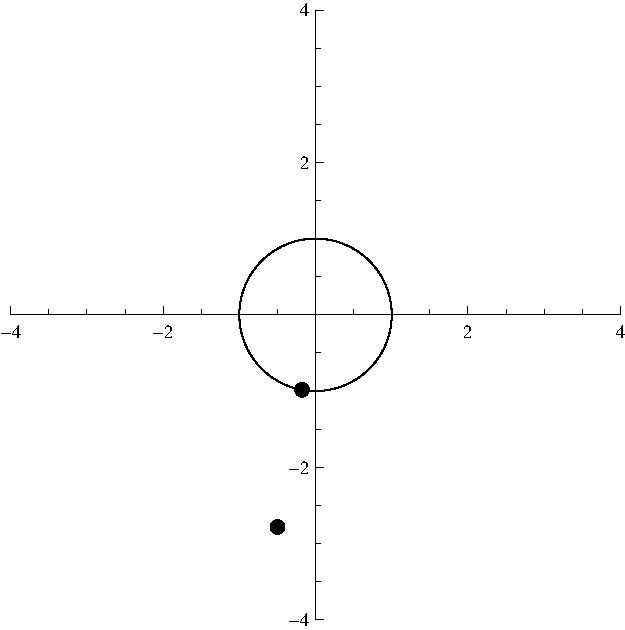
\includegraphics[width=3in]{../graphics/CmplxPlane5.pdf}
\]
Since multiplication of complex numbers lying on the unit circle in the
complex plane is simply rotation, the cube-root of $\frac{-1}{2} + \frac{-\sqrt{31}}{2} i $ is:
\[
\left(\sqrt[3]{2\sqrt{2}}\right)\cos\left(\arcsin\left(\frac{31}{4\sqrt{2}}\right)/3\right) - i \left(\sqrt[3]{2\sqrt{2}}\right) \sin\left( \arcsin\left(\frac{31}{4\sqrt{2}}\right)/3\right)
\]
Plotted on the complex plane, it looks like the black point below:
\[
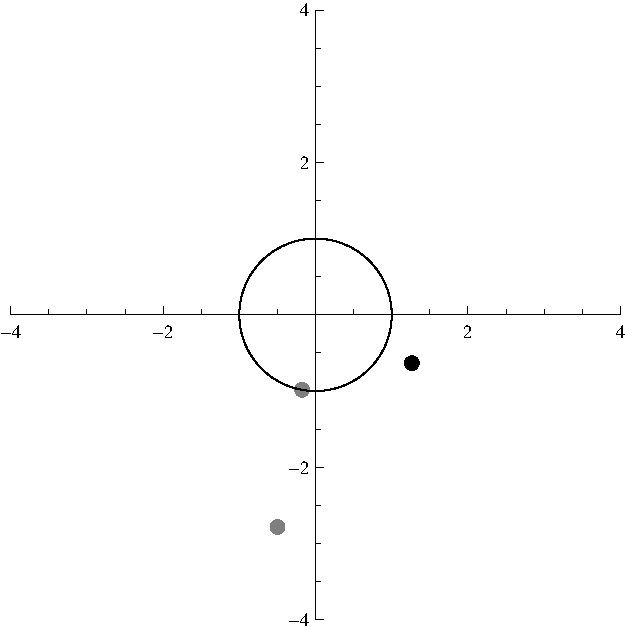
\includegraphics[width=3in]{../graphics/CmplxPlane6.pdf}
\]
Putting all of this together, we find:
\[
\sqrt[3]{\frac{-1+\sqrt{-31}}{2}} + \frac{2}{\sqrt[3]{\frac{1}{2}(-1+\sqrt{-31})}} = \left(2\sqrt[3]{2\sqrt{2}}\right)\cos\left(\arcsin\left(\frac{31}{4\sqrt{2}}\right)/3\right)
\]
A messy, but real, number. 
